\section{System Overview}\label{sec:system-overview}
\subsection{3D-Formatted Data}\label{subsec:3d-formatted-data}
The term "3D-formatted data" is specific to this research, and must be explained to understand the choice of neural network architectures tested.
This is best done by comparing it to "2D-formatted data".

2D-formatted data can be represented as an image, with some horizontal resolution $x$ and vertical resolution $y$.
In this project, each photodiode outputs values at a predetermined sampling rate over the course of a gesture.
This means that we can format said data as a 2D image in which $x$ is the number of photo diodes we use and $y$ is the number of total samples we receive from any of the photo diodes, while the value of each "pixel" in the image is a reading from a single photo diode at a single point in time.

3D-formatted data can meanwhile be thought of as a video, which splits this 2D-image into a sequence of $n$ frames, as shown in figure~\ref{fig:3d-data}\@.
3D-formatting is generally more appropriate when the data is sensitive to time, i.e.\ when data points should be considered in a specific sequence.
Therefore, by 3D-formatting the photo diode data, lower error rates should be achievable as temporal information from the photo diodes isn't lost.

\begin{figure}[h]
    \centering
    \captionsetup{justification=centering}
    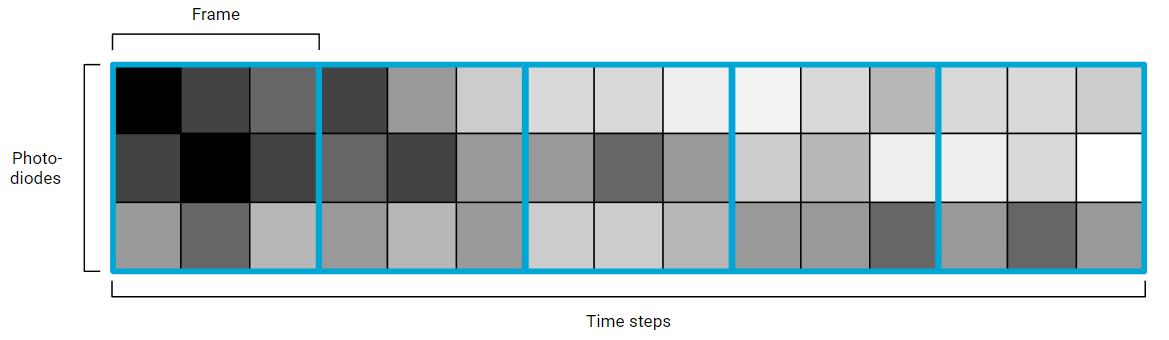
\includegraphics[width=\linewidth]{figures/3d_data}
    \caption{Visualization of photodiode data after 3D-formatting with frame size 3.}
    \label{fig:3d-data}
\end{figure}

\subsection{Full Project Overview}\label{subsec:project-pipeline}
This research focuses on finding an appropriate neural network architecture to perform gesture recognition on a microcontroller, but it is only part of a larger project.
This project is composed of the following tasks:
\begin{enumerate}
    \item Optimizing the number and placement of OPT101 photo diodes.
    \item Reading, processing, and sanitizing data from photo diodes.
    \item Creating an appropriate dataset for training a neural network to recognize gestures.
    \item Finding an appropriate neural network architecture on the created dataset and ensuring gestures can be recognized in real-time on an Arduino Nano 33 BLE\@.
\end{enumerate}

The research presented in this paper aims to complete task 4.
Although tasks 1--3 were completed by other group members and are beyond the scope of this research, they are worth mentioning to provide some context regarding the rest of the gesture recognition system.
Due to the findings from these tasks, the final system uses 3 photodiodes and can recognize 8 different gestures, as illustrated in figure~\ref{fig:system}\@, while each gesture is composed of 100 readings from each photodiode.
This is also relevant for task 4, as it means that whatever architecture is used must use a 2D array of size 3 by 100 as an input feature, and be able to distinguish between 8 output classes.

\begin{figure}[h]
    \centering
    \captionsetup{justification=centering}
    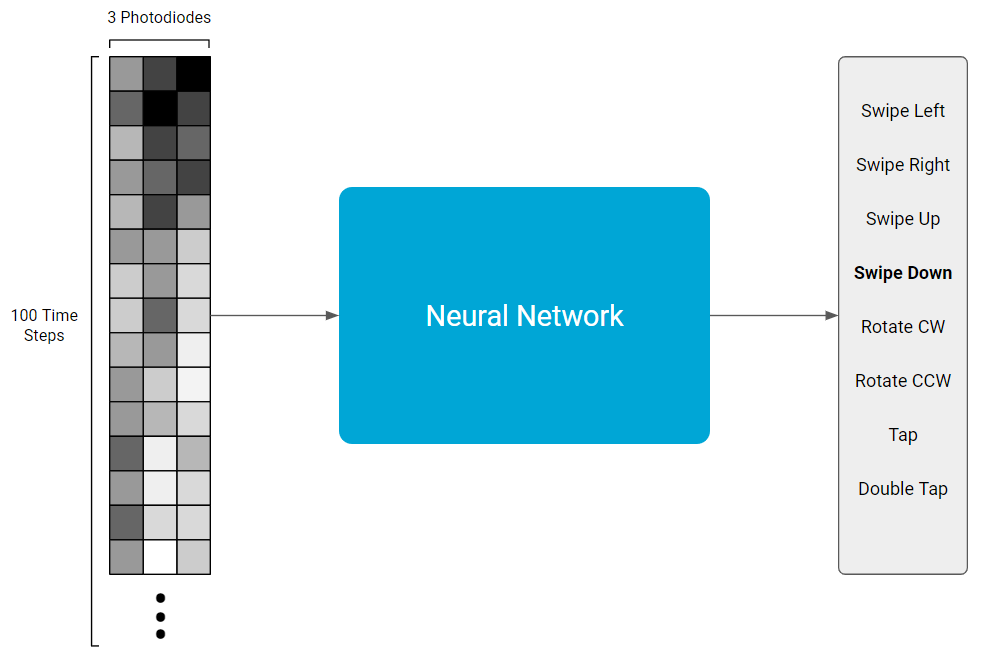
\includegraphics[width=\linewidth]{figures/system}
    \caption{Visualization of the inputs \& outputs of the gesture recognition neural network.}
    \label{fig:system}
\end{figure}
